\documentclass[11pt]{article}
\usepackage[utf8]{inputenc}
\usepackage{graphicx}
\usepackage{hyperref}
\usepackage[a4paper, total={6in, 8in}]{geometry}

\title{Notes on Chapter 5 - Structured Types, Mutability, and High Order Functions}
\author{Swarup Tripathy \thanks{John V Guttag}}
\date{February 2022}


\begin{document}
    \maketitle
    A curated list of important points for my reference.\\
    \begin{enumerate}
        \item Literals of type \textbf{tuples} are written by enclosing a comma separated list of elements within parenthesis.
        \item Like strings, tuples can be concatenated, indexed and sliced.
        \item Sequences and Multiple Assignments
        \begin{itemize}
            \item Executing the statement x,y=(3,4) where x will be bound to 3 and y to 4
            \item The statement a,b,c = 'xyz' will bind x to a, y to b and z to c.
        \end{itemize}
        \item Built-in-function \textbf{id}, which returns a unique integer identifier for an object.
        \item Deep and Shallow copy in python
        \begin{verbatim}
            import copy
            copy.copy(x)        #shallow copy
            copy.deepcopy(x)    #deep copy
        \end{verbatim}
        \begin{itemize}
            \item Shallow Copy $\rightarrow$ A shallow copy creates a new object which stores the reference of the original elements.
            So, a shallow copy doesn't create a copy of nested objects, instead it just copies the reference of nested objects. This means, a copy process does not recurse or create copies of nested objects itself.
            \centering
            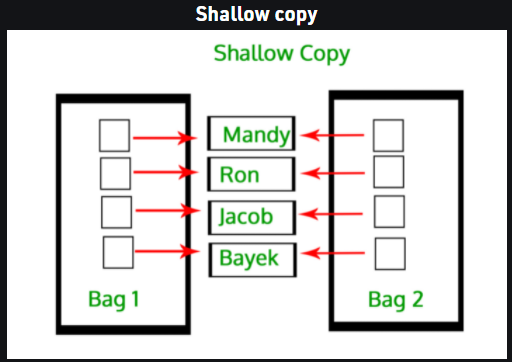
\includegraphics[width=4.5cm]{imgs/2.png}

            \item Deep Copy $\rightarrow$ A deep copy creates a new object and recursively adds the copies of nested objects present in the original elements.
            The deep copy creates independent copy of original object and all its nested objects.
            \centering
            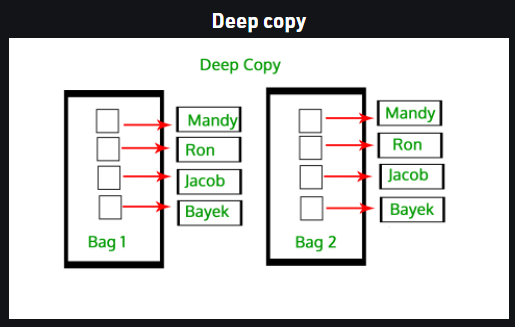
\includegraphics[width=5cm]{imgs/1.png}
        \end{itemize}
        \item Python supports creation of anonymous functions (i.e., functions which are not bound to a name), using the reserved word \textbf{lambda}. The general form of a lambda expression is
        \begin{verbatim}
            lambda <sequence of variable names>: <expression>

        L=[]
        for i in map(lambda x,y: x**y,[1,2,3,4],[3,2,1,0]):
            L.append(i)
        print(L)

        prints out [1, 4, 3, 1]
        \end{verbatim}
        \item IMMUTABLE datatypes (e.g. int, float, bool, str, tuple, unicode) cant be changed after they are created, 
        \item MUTABLE datatypes (e.g. list, set, dict, byte array) can be changed. An object whose internal state can be changed is mutable
        \item In python programming, the second name given to a piece of data is known as an alias. Aliasing happens when the value of one variable is assigned to another variable because variables are just names that store references to actual value.
        reference: \href{https://www.codesansar.com/python-programming/aliasing.htm#:~:text=In%20python%20programming%2C%20the%20second,store%20references%20to%20actual%20value.&text=So%2C%20both%20variables%20point%20to,same%20string%20object%20'PYTHON'.}{Aliasing}
        \item Dictionary being as set of key/value pairs. Literals of type dict are enclosed in curly braces
        and each element is written as a key followed by a colon followed by a value.
        \item Like lists, dictionaries are also mutable
    \end{enumerate}
\end{document}